\section{Voice}

Voice is the most common feature describing the predicate. It describes the relationship between the action the predicate expresses and the participants of the action (the subject, objects etc.).

There are three voices in Novoslovnica:

\begin{itemize}
	\item Active
	\item Reflexive
	\item Passive
\end{itemize}

\begin{figure}
	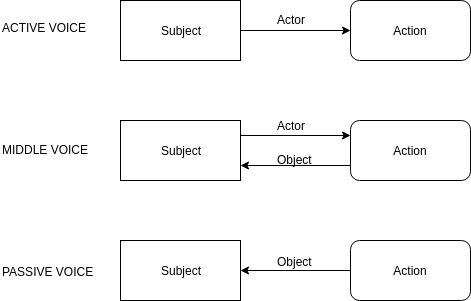
\includegraphics[width=\linewidth]{./sources/voices.png}
	\caption{Voices in Novoslovnica}
	\label{fig:voices}
\end{figure}

\textbf{Active voice}

The active voice describes a sentence where the subject performs the action stated by the verb.

\underline{Examples:}

\textit{Moǐ brat sę zova Ivan.} - My brother's name is Ivan.

\textit{Glědaǐ u prozorec!} - Look at the window!

\textbf{Reflexive voice}

The reflexive voice describes a sentence where the subject plays the both the role of the actor and the object.

\underline{Examples:}

\textit{Ja sę učim govoriti anĝliǐskym jazykom.} - I learn how to speak English.

\textit{On sę glědaje v zòrcadlo.} - He is looking at himself in the mirror.

\textbf{Passive voice}

The passive voice describes a sentence where the action stated by the verb is acted over the subject.

\underline{Examples:}

\textit{Ryba je byla zjědena kotom.} - The fish was eaten by a cat.

\textit{Moǐ prijatelj je byl prijęt do råboty.} - My friend was accepted for the job.